\chapter{Design}
\label{chap:design}

The focus of the thesis are the questions asked in Section~\ref{sec:research_questions_and_methodology}. We asked ourselves how we can verify convergence happens for context models, access groups and services with the S2Store. We looked into DS2OS (Section~\ref{sec:ds2os}) and how it provides portability (Section~\ref{sec:portability}). S2Store allows us to achieve portability through convergence (Section~\ref{sec:portability}). We analyzed app stores and their features (Section~\ref{sec:introduction_to_an_app_store}). We analyzed what reputation systems are, how they are put together and how they function (Section~\ref{sec:reputation_systems}). We analyzed how app stores can be studied with the help of simulation (Section~\ref{sec:analysis_appeco}). We finally analyzed the S2Store ecosystem and explained what convergence mechanism are and what benefits they provide (Section~\ref{sec:s2store_ecosystem}). 

In the following sections, we describe the elements we borrow from our analysis to answer our research questions.

\section{Modified AppEco for S2Store : Introduction}
\label{sec:s2eco}

An S2Store is also an app store because it shares the same features and requirements as found in the general definition presented by \cite{Jansen}. Like in a mobile app store, S2Store has users and developers. The difference is that while in a mobile app store, developers and users engage through apps, in S2Store they engage through services. Services are more complex compared to apps because of lack of standards and portability reasons (Section~\ref{sec:portability}). S2Store not just hosts one type of entity: services but also other entities like context models and access groups (Section~\ref{sec:s2store_ecosystem}).

AppEco simulation has provided with valuable insights in answering questions related to app stores. We extend AppEco for S2Store by introducing a similar simulation called \emph{S2Eco}. Through S2Eco, we observe the behavior of the smart space ecosystem and try to find the answers of our questions. Significant parts of the AppEco simulation has been explained in Section~\ref{sec:analysis_appeco}. With this as base, we expand the simulation to suit for S2Store. The additions and changes are explained in the following sections.

Like AppEco, S2Eco consists of artificial model agents. In addition to developer and user agents, S2Eco contains artifacts like services, context models and access groups instead of apps in AppEco. Developer agents develop services with corresponding context models and access groups and upload them to the S2Store. Users browse the S2Store and download the services. Users can then provide positive or negative feedback about the services online.

Each entity and its interactions are explained in the following section:

\section{Developer Agents}

The developer agent in S2Eco has all of the behavior of the developer agent in AppEco. But instead of building apps, they build services. Each developer agent requires \emph{devDuration} days to build a service such that: $$devDuration \in [dev_{min}, dev_{max}]$$

Each developer is initially active and continues to build and upload the services. However she has a chance to become inactive with a probability of $P_{inactive}$. This models hobbyist, part-time developers, and the tendency of developers to stop building services. Each developer uses one of the following strategies to build the services:

We could model a developer to alter between the four strategies described in AppEco (Section~\ref{subsubsec:appeco_components_developers}): S0 Innovator, S1 Milker, S2 Optimizer or S3 Copycat. There is however a significant difference here: mobile app stores are more competitive marketplace than cooperative and collaborative platform. In contrast; for S2Store, collaboration is a significant element (Section~\ref{sec:portability}). Specially for developers, we assume that developers behavior are more collaborative and less competitive \cite{dabbish2012social}. Hence in S2Eco, we only consider S0 Innovator and ignore the rest of the strategies.

Due to feedback mechanism available in app stores, developers are constantly notified with the feedbacks received from users. The way by which they react to the feedbacks are different. We create three different categories to place the developers based on their possible reactions to feedbacks: \emph{Improver}, \emph{Ignorer} and \emph{Malicious}.

\begin{itemize}
  \item \textbf{Improver} fixes all the bugs from the applications she owns. This models the individuals who improve their applications constantly.
  \item \textbf{Ignorer} do not care about the feedback. This models developers who submit their application once and chooses not to improve them regardless of feedback from users.
  \item \textbf{Malicious} developers are those who add additional bugs into their software. They model beginner developers who are not proficient with development. This also models developers who intentionally add malicious features to the apps once these apps get famous.
\end{itemize}

\emph{Hypothesis 1} Depending upon the category of a developer, the average rating of the services has distinct behavior per category. Services by \emph{Improvers} should have strong improvement on rankings over time and should cause higher downloads. Services by \emph{Ignorers} should show a constant or slightly decreasing average ratings over time. Services by \emph{Malicious} developers should show decrease in rankings over time.

\emph{Hypothesis 2} The ratings of context models and access groups would strongly correlate for \emph{Improvers} because popularity of services bring visibility to the associated context models and access groups. The chance that other developers also use the context models increase with increased visibility. However since context models are immutable, decrease in ranking of services due to \emph{Ignorers} and \emph{Malicious} developers should not affect the reputation of already uploaded context models.

\section{Services}

A service entity models an actual service uploaded in the real S2Store. It is modeled exactly similar to an app in AppEco. It is built and uploaded to the S2Store by developer agents. The features of a service are abstracted as a 10x10 feature grid $F_s$ for each service. Each cell in the 10x10 grid is a feature. If a cell is filled in $F_s$, then the service offers that particular feature.

The service feature grid $F_s$ is filled with a probability of $P_{featS}$ as shown in Figure: \ref{fig:example-service-grid}.

\begin{figure}[!htb]
  \centering
  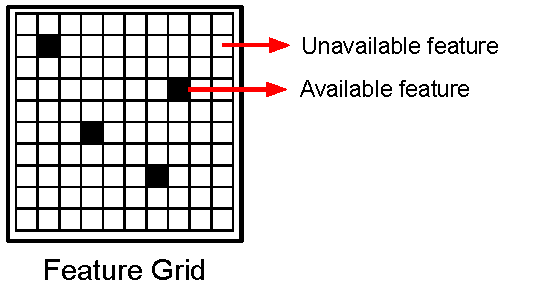
\includegraphics[width=9cm]{figures/example_service_grid.pdf}
  \caption{Example of a service grid. Each cell is filled with a probability of $P_{featS}=0.04$. A cell filled with black at row=r and col=c represents that it has a feature at coordinate r,c}
  \label{fig:example-service-grid}
\end{figure}

Various types of services have been discussed in Section~\ref{subsec:access_groups_and_convergence}. For artificial life simulation, we remove the differences between them and generalize all services to behave in one simple way: their features are randomly generated.

A service entity stores the day when it was created to identify if it is a new service or not. 

In S2Eco, service entities have two major roles.

\begin{enumerate}
  \item They store reputation scores calculated by S2Store. These scores change over time. The change in score is measured and analyzed (Section~\ref{sec:experiments}).
  \item Service entities dictate the popularity of context models by virtue of their inter-relationship. The more service entities use a context model, the popular it becomes in comparison to other context models. We also observe this behavior in S2Eco (Section~\ref{sec:experiments}).
\end{enumerate}

\section{Devices}
\label{sec:devices}

A device entity models the presence of wide variety of devices in the market. A device model represents the abstract concept of the utility of the device. For example, A washing machine is an abstract concept with predefined set of utilities (should be able to wash clothes, should have a connector to water supply, etc). But we can find different designs, brands and models of washing machines in the market. Here, the device entity would model the concept of a washing machine.

Devices entities are associated with Context Model entities discussed below. Ideally for portability reasons, each device would have one context model. But crowd sourced development means different developers come up with their own designs that fit their purpose. A device entity can be associated with many different services.

\section{Context Models}
\label{sec:context_models}

Context models have been explained in Section~\ref{subsec:cmr}. They abstract the context in a physical world into the virtual world. When a developer designs a service, the service uses the context models to communicate with different devices and other services. So a service is always associated with at least one context model, if not many.

A developer writes down the list of context models her service uses before packaging the service and uploading it to the S2Store. Context model entities in S2Store save the relationship between context models and services. In each timestep of the simulation, the number of relationships between services and devices are counted to give a popularity ranking to the context models. The more a context model is associated with different services, the more popular it is.

Whenever a developer thinks about creating a service, she starts with the problem. She then identifies the solution and the list of devices she can use to build the solution service. She goes on to the S2Store and checks the CMR for a list of context models suitable for the device. The S2Store will show her all similar context models that suit her device along with the reputation score of each context model.

It does not always have to be a device for a developer to search a context model. Context models can represent other abstract concepts, act as a common data store, etc independent of any association with physical devices. However, for simplicity reasons, we assume all context models are derived from devices.

Thus, all context models in S2Eco are also associated with devices. By default, a context model is always associated with one device in the simulation while this is not necessary in real world. This has been done again to simplify the simulation.

Context models are also associated with other context models as they form hierarchical structures. Simple context models that represents simple devices are combined together to describe a complex context model that represents a complicated device. For e.g., a context model for an automated window will depend upon context models for automated hinges, open and close switch for window blinds, ambient light and wind sensors etc. Second, a developer has to specify in any service she develops, which context models the service is dependent upon. For e.g., an automated window control service will specify context models for a temperature sensor and on/off switch control. These two context models have an internal connection in the system.

We also assume that context models evolve over time. At the beginning when the platform has not gained wide spread adoption with developers, context models are simpler: have less features. With time, context models with higher complexity are created.

The features in a context model are also abstracted as a 10x10 feature grid $F_{cm}$ as with apps in AppEco (Section~\ref{subsubsec:apps}). Each cell of a $F_{cm}$ is filled with a probability of $P_{featCM}$. In contrast to the fixed probability value $P_{Feat}$ for apps in AppEco or the probability value of $P_{featS}$ of the services, the probability of a context model $P_{featCM}$ is a linear function of timesteps. As time progresses, $P_{featCM}$ increases as shown in Eq.~\ref{eqn:linear_context_model_function}.

\begin{equation}\label{eqn:linear_context_model_function}
P_{featCM}(t) = P_{featCMmin} + \frac{P_{featCMmax} - P_{featCMmin}}{T_{total}} * t
\end{equation}

Where, $T_{total}$ is the current timesteps or total number of days for simulation.

\begin{figure}[!htb]
  \centering
  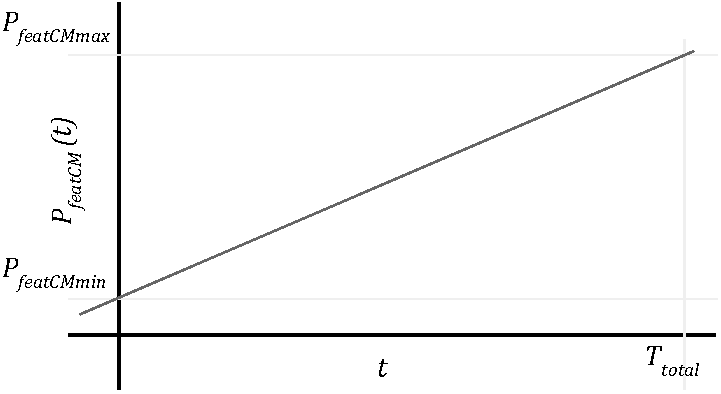
\includegraphics[width=12cm]{figures/probability-of-feature-vs-time.pdf}
  \caption{Linear relationship between $P_{featCM}(t)$ and time $t$.}
  \label{fig:probability-of-feature-vs-time}
\end{figure}

\begin{figure}[!htb]
  \centering
  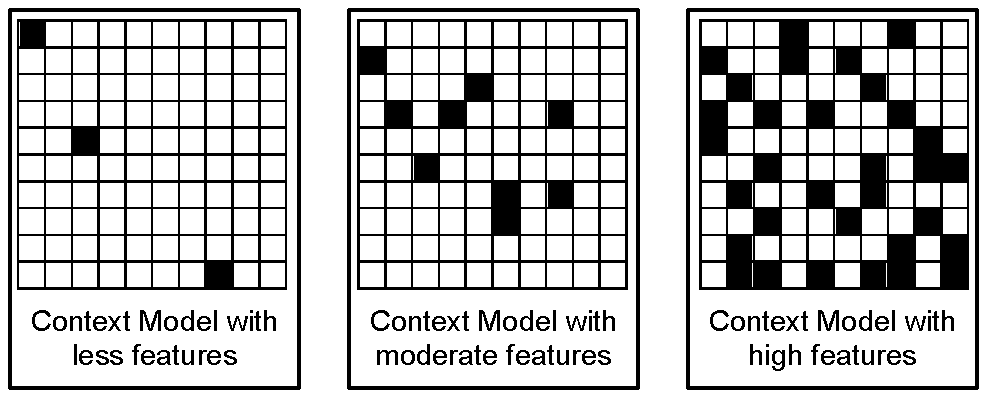
\includegraphics[width=12cm]{figures/feature-level-of-context-models.pdf}
  \caption{Amount of features of context models increase with time.}
  \label{fig:feature-level-of-context-models}
\end{figure}

Linear growth of $P_{featCM}(t)$ with time $t$ can be seen in Figure~\ref{fig:probability-of-feature-vs-time}. It results in context models getting more complicated over time as shown in Figure~\ref{fig:feature-level-of-context-models}. There are three context models with increasing number of filled black cells from left to right. The context model on the left is the least complex and the one on the right is the most complex in terms of number of features.

We assume that simpler context models have less dependencies with other context models while complex context models have higher dependencies with other context models.

To illustrate this, we take an example of two context models. A simple automatic lamp can depend upon \emph{an ambient light sensor}, \emph{a switch}, \emph{own light source}. A complex room automation system depends upon a lot of context models of higher abstractions like \emph{lighting}, \emph{temperature control}, \emph{music and multimedia control}, \emph{personal assistance} etc which themselves are complex and depend upon lower abstractions.

We model this behavior such that a context model with $x$ features depends upon $N$ other context models where $N$ is given by,

Given $\textbf{Y}$ is a random independent variable,
\begin{equation}
  \begin{aligned}
    Y &\in [0, 1],\\
    N &= Y * f(x),\\
    f(x) &= N_{min} + \frac{N_{max} - N_{min}}{100} * x
  \end{aligned}
\end{equation}

\begin{figure}[!htb]
  \centering
  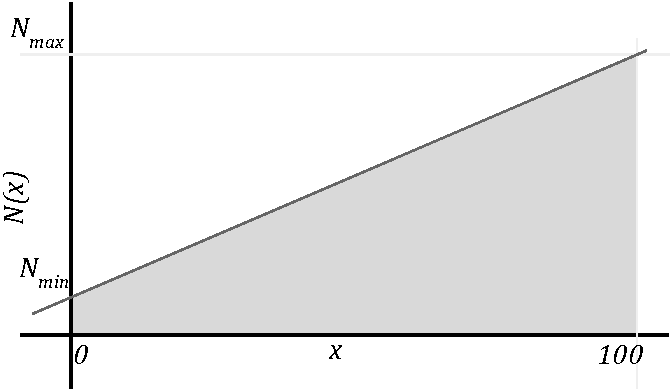
\includegraphics[width=12cm]{figures/num-of-context-models-vs-features.pdf}
  \caption{The gray portion represents the number of context models $N(x)$ associated with a new context model with $x$ number of features. A complex context model with large features has probability to have higher number of related context models.}
  \label{fig:num-of-context-models-vs-features}
\end{figure}

\begin{figure}[!htb]
  \centering
  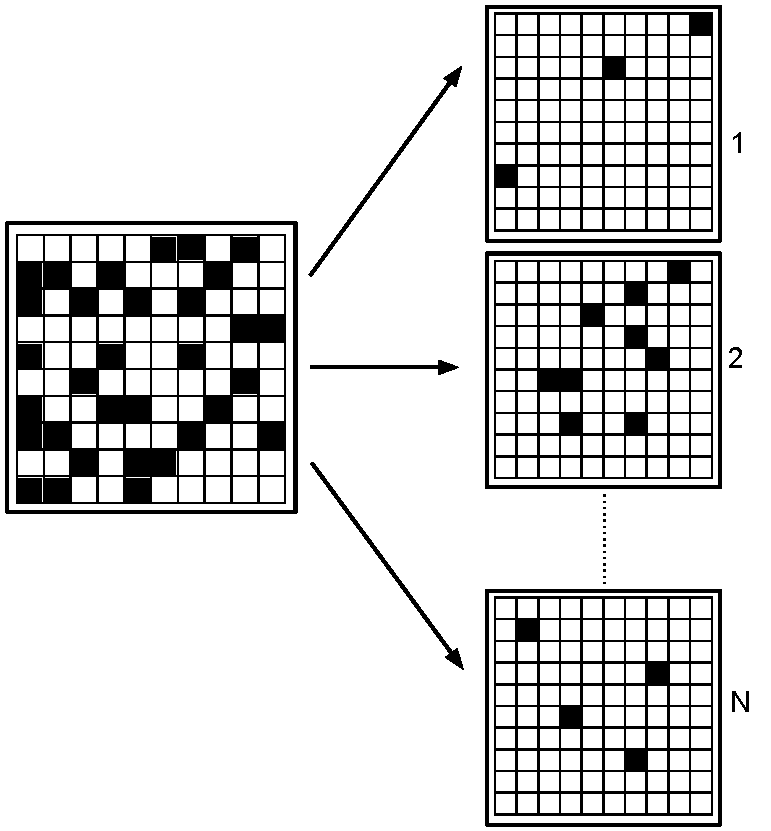
\includegraphics[width=8cm]{figures/context-model-dependency.pdf}
  \caption{A context model dependent upon N other context models.}
  \label{fig:context-model-dependency}
\end{figure}

The increase in context dependencies from one context to another is shown in Figure~\ref{fig:num-of-context-models-vs-features}. Figure~\ref{fig:context-model-dependency} shows a context model on the left dependent upon $N$ other context models on the right.

By modeling increase in complexity of context models and the increase in dependency of a context model to other context models, we assume that S2Eco is slowly evolving over time. We used the linear growth as suits better than other models because it gives more predictable result during simulation.

\subsection{Ranking of Context Model}

In real world S2Store, developers search for these dependent context models. They have a particular feature requirement and search for other context models that provide these features. Developers can search by category or by text. The search results are ordered according to the ranking of each context model.

\begin{figure}[!htb]
  \centering
  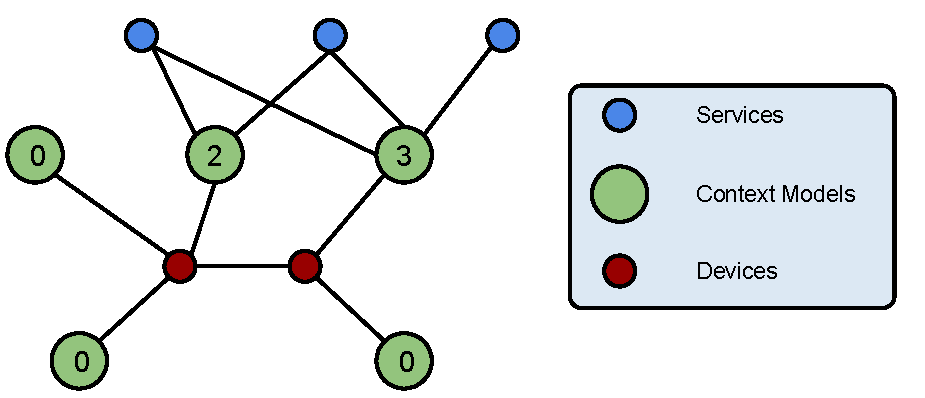
\includegraphics[width=10cm]{figures/association_between_context_models.pdf}
  \caption{Association between context models through services. The numbers inside the context models show the \emph{Reputation Value}.}
  \label{fig:association-between-context-models}
\end{figure}

Ranking of a node determines its popularity. Associations between context models can be modeled in a graph where each context model is a node and the association with other context models is represented as a edge as shown in Figure \ref{fig:association-between-context-models}. Popularity of a context model is calculated as a centrality measure. Different centrality measures exist. In S2Eco, we use the number of services that use a context model as its reputation score. For e.g., if 15 services mention context model $c$, then $R(c)=15$ where $R$ is a reputation function.

\subsection{Algorithm of how a developer chooses a context model}

An active developer when creating a new service, decides on the devices she wants to associate in the service. The number of devices for a service is chosen randomly between [1, $D_n$] where $D_n$ is a function dependent upon the simulation timesteps. As timesteps increase, a developer is likely to choose more devices for her services.

This is based on the expectation that at the beginning of the ecosystem, most of the services contributed are likely to be adaptation services that allow future services to take advantage of real world devices. In future, the number of devices associated per service increases.

She then searches the S2Store for existing context models matching the devices. She is either satisfied and chooses the existing context model or she is unsatisfied and decides to create her own new context model.

A device ends up having multiple context models. When a developer searches for existing context model, we want her to be able to find the one which is used the most by other developers. This behavior is simulated such that the probability of a developer choosing a particular context model depends upon how many existing services already use it. The probability distribution is given by $$P_{selectCM}(x)=\left\vert{E(x,y)}\right\vert$$ where $E(x,y)$ is a set of all associations of the context model $x$ with any existing services. A context model is five times more likely to be picked by a developer if it is already used by five existing services than another context model that is used by only one existing service.

\section{User Agents}

Each user agent has preferences that determine the service features that it prefers, similar to user preference in AppEco. The preferences of a user agent are also abstracted as a 10x10 preferences grid ($\textbf{U}$). The cells in $\textbf{U}$ are filled probabilistically, such that each cell in the grid has a probability of $P_{Pref}$ of being filled. If a cell in $\textbf{U}$ is filled, then the user agent desires the feature represented by that cell. If the feature grid of a service $F_s$ has a cell in the same location filled, then it means the service offers a feature desired by the user agent. In Figure \ref{fig:user-service-feature-matching}, all four of the features offered by Service 1 match the user agent's preferences, but only two of the features offered by Service 2 match the user agent's preferences. The matching is binary, so either the cells match or do not match.

\begin{figure}[!htb]
  \centering
  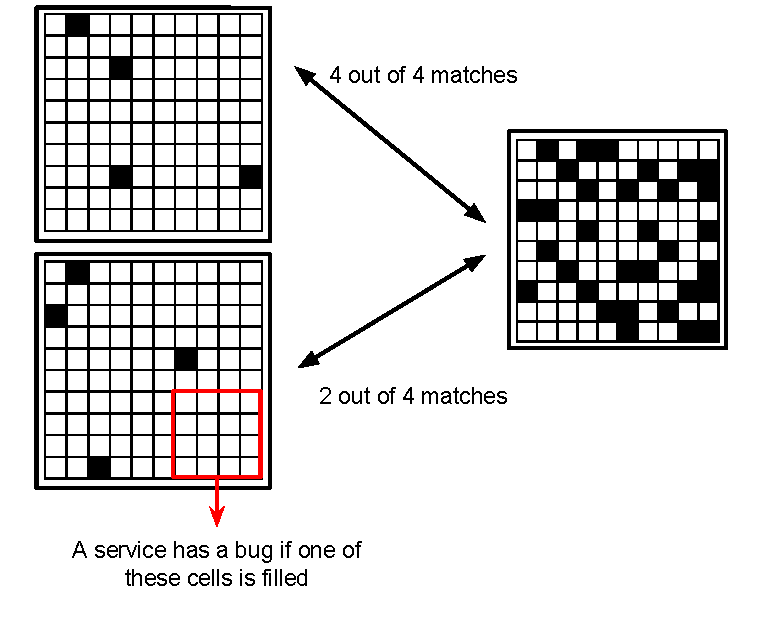
\includegraphics[width=10cm]{figures/user_service_feature_matching.pdf}
  \caption{Matching service features with user preferences}
  \label{fig:user-service-feature-matching}
\end{figure}

A user agent keeps record of the number of services it has downloaded and the number of days between each browse of the S2Store ($daysBtwBrowse$, a random value between $[bro_{min}, bro_{max}]$), and the number of days that have elapsed since it last browsed the S2Store ($daysElapsed$). $daysElapsed$ is recorded so that the user agent knows when to browse the app store next. When a user is initialized, the $daysElapsed$ is set to a random number between $[0, daysBtwBrowse]$ so users don't all browse at the same time when they start.

\section{S2Store}

S2Store is used by the agents to store and access \emph{Context Models} and \emph{Services}. For developers, it allows to see access groups and context models uploaded by other developers. Developers can search for a context model based on number of features as explained in \ref{sec:context_models}.

Users can use the S2Store to browse the services. There are three methods for browsing: Top Services Chart, New Services Chart, Keyword Search. Top Services Chart lists the services based on their reputation. New Services Chart lists the services based on the date of upload (latest services appear at the top). Keyword search is abstracted as random search for random service.

\section{Algorithm}

Our algorithm based on the AppEco algorithm from \cite{lim2012successful}. It models the interaction between the components described in previous sections. Each timestep in the algorithm represents a day in the real ecosystem.

Population growth of the developers and users is modeled using a sigmoid growth function commonly used to model the population growth in natural systems. The equation models the growth rate of users and developer agents in an app ecosystem declining as their population density increases. The population size at timestep $t$, $pop(t)$ is defined by 

\begin{equation}\label{eq:s2eco_algorithm}
  pop(t)=MinPop + \frac{MaxPop - MinPop}{1+e^{S*t-D}}
\end{equation}

where $MinPop$ is the minimum population, $MaxPop$ is the maximum population, $S$ determines the slope of the growth curve and $D$ shifts the curve from left to right.

The algorithm is shown in Figure \ref{fig:algorithm-flow} and explained below:

\begin{figure}[!htb]
  \centering
  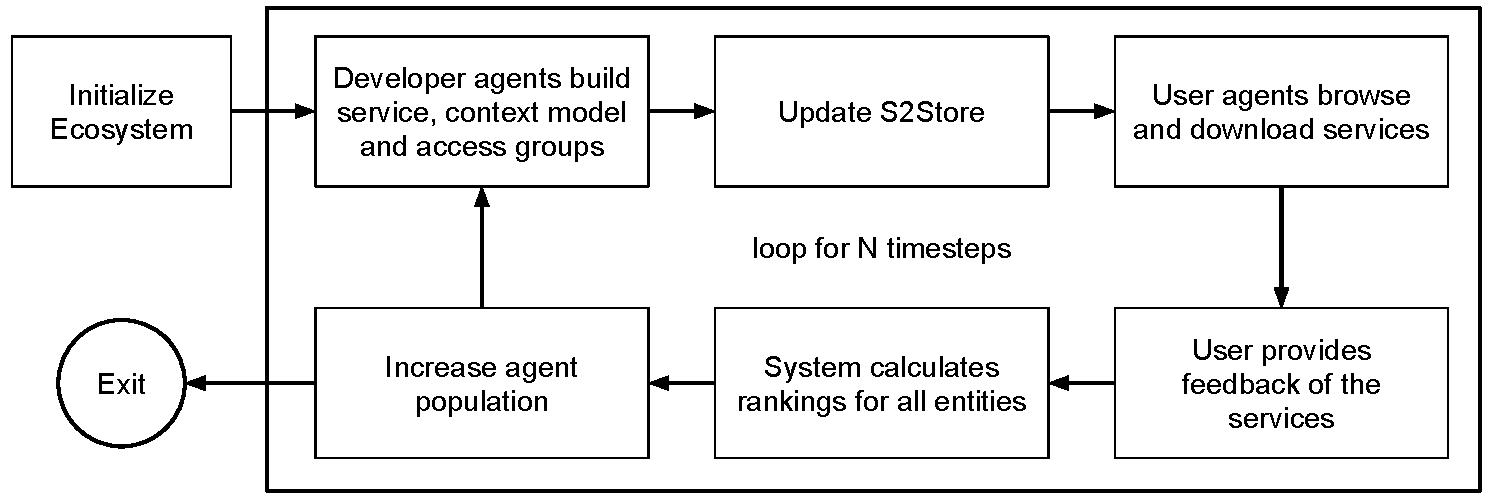
\includegraphics[width=13cm]{figures/algorithm-flow.pdf}
  \caption{Matching service features with user preferences}
  \label{fig:algorithm-flow}
\end{figure}

\subsection{Initialize ecosystem}

The step launches S2Eco with the population of developer and user agents as defined in \ref{eq:s2eco_algorithm}, with timestep = 0.

\subsection{Developer agents build services, context models}

For each active developer, \emph{daysTaken} is incremented by 1. If \emph{daysTaken} exceeds the developer's \emph{devDuration}, the development of service is completed. Developer then uploads the service to the store, resets \emph{daysTaken} to 0, and decides on the next service to build. The feature grid $F$ of the service is set as described earlier.

Any new context models created when creating the service are also uploaded to the S2Store.

The developer also goes through her old services to see if they have bugs as reported from the users. The developer then acts according to his nature. \emph{Innovator} removes the bugs, \emph{Ignorer} ignores the bugs while \emph{Malicious} user introduces new bugs. The modified services are then uploaded to the S2Store.

\subsection{Update S2Store}

New Services Chart contains $T_{newServices}$ number of latest uploaded services ordered by the latest service on top. Top Service Chart list is also updated so that services are ranked in the order of decreasing score, calculated as $8*D_1+5*D_2+5*D_3+3*D4$ where $D_N$ is the number of downloads received by the service on the \emph{n}th day before the current day.

\subsection{User agents browse and download services}
For each user, \emph{daysElapsed} is incremented by 1. If \emph{daysElapsed} exceeds \emph{daysBtwBrowse}, then the user browses the S2Store, and resets \emph{daysElapsed} to 0. User browses New Services Chart and the Top Services Chart as well as conducts Keyword Search. Keyword Search returns a random number of services from the S2Store. User filters through all the services by matching her preference grid with the feature grid of the services. For e.g., in Fig \ref{fig:user-service-feature-matching}, the user downloads Service 1 but not Service 2.

\subsection{User agents provide feedback of the services}

In this step, all users who browsed the S2Store goes through their newly downloaded services. If a service has a bug, the user votes randomly between 1 and 2. If a service has no bug, the user votes randomly between 3,4 and 5.

\subsection{System calculates rankings for all entities}

This step calculates and stores the average rating of all the services.

\subsection{Increase agent population}

This step increases the number of devices, users and the developers in S2Eco for the next time step, using Eq. 1.

\section{Discussion}

We now have a structure for the S2Eco simulation. It contains all the basic necessary elements that interact with one another: developers, users, services, context models and access groups. There are limitations to the simulation because in real life, the behaviors are very complex. We have not attempted to capture many of these complexities. We have a basic system with the smallest amount of features that allow us to answer our questions.

The simulation focuses on the quality of services delivered by the users and the kind of user feedbacks provided back into the system. This should show us interesting patterns in terms of increased ratings and increased number of downloads. The simulation also focuses in popularity of context models depending upon the number of services that use a particular context model or inter context model relationships. By altering the nature of how these inter-relationships occur, we can see how the relationships evolve and how soon a context model becomes popular among other similar competing context models.